% LNL PAC proposal, Jan 2027 call -- MX17 two-arm X17 feasibility study.
% Rules (lnl.infn.it/en/details-for-submissions): abstract <= 1 page (not counted);
% body <= 5 pages, 12 pt, figures/tables/references included.
% When the official LNL template is downloaded from Indico (event 50487), move the
% text below into it; the section structure already follows the rules.
\documentclass[12pt,a4paper]{article}
\usepackage[margin=2.0cm]{geometry}
\usepackage[T1]{fontenc}
\usepackage[utf8]{inputenc}
\usepackage{lmodern}
\usepackage{amsmath,amssymb}
\usepackage{graphicx}
\usepackage{booktabs}
\usepackage{xcolor}
\usepackage{tikz}
\usepackage{siunitx}
\usepackage[hidelinks]{hyperref}
\usepackage{enumitem}
\usepackage{caption}
\captionsetup{font=small,labelfont=bf}
\setlist{nosep,leftmargin=1.2em}
\sisetup{range-phrase=--,range-units=single}

% Draft markers: \todo{...} shows in red; set \drafttrue to \draftfalse to hide them.
\newif\ifdraft \drafttrue
\newcommand{\todo}[1]{\ifdraft\textcolor{red}{[#1]}\fi}
\newcommand{\Be}{\ensuremath{^{8}\mathrm{Be}}}
\newcommand{\Li}{\ensuremath{^{7}\mathrm{Li}}}
\newcommand{\pee}{\ensuremath{(p,e^+e^-)}}
\newcommand{\Xs}{X17}

\begin{document}

%======================================================================================
% ABSTRACT PAGE (one page, not counted)
%======================================================================================
\thispagestyle{empty}
\begin{center}
{\Large\bfseries Feasibility study of an X17 search in \Li\pee\Be\\[2pt] with the MX17 Micromegas-TPC spectrometer}\\[10pt]
{\large Proposal to the LNL PAC, January 2027}
\end{center}
\vspace{4pt}
\begin{tabular}{@{}p{0.28\textwidth}p{0.68\textwidth}@{}}
\textbf{Accelerator} & AN2000 (alternative: CN) \\
\textbf{Experimental set-up} & MX17, two-arm configuration (Micromegas TPC + SiPM scintillator wall + plastic scintillators per arm), around a \Li{} target at the end of a beam line \\
\textbf{Beam} & protons, $E_p = 0.441$ and $1.10$~MeV, up to 1~\si{\micro\ampere}, continuous \\
\textbf{Beam time} & 8 days, second half of 2027 \\
\textbf{Spokesperson(s)} & \todo{to decide: D.~Neff / P.~Mastinu} \\
\textbf{GLIMOS} & \todo{local, to decide} \\
\end{tabular}

\vspace{6pt}
\noindent\textbf{Authors.}
D.~Neff\textsuperscript{1}, P.~Mastinu\textsuperscript{2},
\todo{C.~Massimi, A.~Mengoni, G.~Gervino, C.~Gustavino, L.~Cosentino, \dots: names and affiliations to confirm}

\vspace{2pt}
{\small
\textsuperscript{1}\todo{affiliation}\quad
\textsuperscript{2}INFN, Laboratori Nazionali di Legnaro, Legnaro (PD), Italy\quad
\todo{others}}

\vspace{8pt}
\noindent\textbf{Summary.}
The anomaly reported by ATOMKI in the opening-angle distribution of $e^+e^-$ pairs from the 18.15~MeV
$1^+$ state of \Be{}, interpreted as a new boson of about 17~MeV (\Xs), has been neither confirmed nor
excluded: a two-arm spectrometer in Hanoi reported a similar excess, MEG~II found none, and a 2026
study showed that cosmic rays alone can produce a bump near $140^\circ$ in ATOMKI-type spectrometers.
The MX17 apparatus, built for and operated in 2026 at CERN n\_TOF, tracks each lepton in a large
Micromegas time projection chamber in front of a scintillator wall and plastic scintillators. It
measures the pair opening angle from the hit positions, rejects cosmic rays by their straight,
collinear tracks, and covers about 40\,\% of the solid angle for the \Xs{} pairs with four arms, against
a few per cent for scintillator telescopes.

We propose an 8-day feasibility study with two opposite arms of the apparatus around a thin metallic
\Li{} target on AN2000: (i)~rates, live time and detector occupancy on a proton beam; (ii)~a calibration
of acceptance, angular resolution and energy scale on the 17.64~MeV M1 transition at the 441~keV
resonance, where no anomaly is expected; (iii)~a measurement of the cosmic-ray and beam-induced
backgrounds with and without the tracking veto; and (iv)~a first look at the 18.15~MeV region at
$E_p = 1.10$~MeV, with an expected sensitivity at the level of the ATOMKI signal and of the MEG~II limit.
The results will fix the design and the beam request of the full four-arm experiment.

\newpage
\setcounter{page}{1}

%======================================================================================
% BODY (max 5 pages incl. figures, tables, references)
%======================================================================================
\section{Scientific motivation}

In 2016 the ATOMKI group observed an excess of $e^+e^-$ pairs at large opening angles
($\theta \approx 140^\circ$) in the decay of the 18.15~MeV $J^\pi = 1^+$ state of \Be{}, populated in
\Li$(p,\gamma)$ at $E_p \approx 1.04$~MeV~\cite{Kra16}. The excess is consistent with the emission of a
neutral boson of mass $m_X \approx 16.7$~MeV with a branching ratio
$R = \Gamma_X/\Gamma_\gamma \approx 5.8\times10^{-6}$. Similar anomalies were later reported in \textsuperscript{4}He and
\textsuperscript{12}C~\cite{Kra21}, and in the \Be{} direct-capture region~\cite{Sas22}. An independent two-arm
spectrometer built in Hanoi with ATOMKI reported a $>4\sigma$ excess at $E_p = 1.225$~MeV~\cite{Anh24}.

The MEG~II collaboration measured the same reaction with its large tracking detector and found no
signal, setting $R(18.15) < 1.2\times10^{-5}$ at 90\,\% CL~\cite{MEG24}. In 2026, members of MEG~II showed
with a full simulation of the ATOMKI spectrometers that cosmic-ray coincidences produce a structure
near $140^\circ$ in the \Be{} energy window, comparable to the IPC itself at ATOMKI running
conditions~\cite{MEG26}. The question is therefore open, and the decisive experimental requirements are
clear: \emph{measured} lepton directions, a strong and \emph{demonstrated} rejection of cosmic rays, a
calibration of the angular response on a transition without anomaly, and enough acceptance to reach
the ATOMKI branching ratio with a margin. At LNL, a scintillator-telescope pair spectrometer has taken
data on AN2000 in 2023--24~\cite{GS25}; a tracking measurement would be complementary.
\todo{one sentence after talking to the LNL \Be{} group (T.~Marchi et al.)}

The MX17 apparatus was built for the search for \Xs{} in $^3$He$(n,e^+e^-)^4$He at CERN n\_TOF, where it
took data in 2026~\cite{Gus20}. Its arms combine a Micromegas TPC, which measures the lepton position to
0.6--0.8~mm, with a scintillator wall and plastic scintillators for triggering and energy. Ported to a
low-energy proton beam, it addresses exactly the requirements above: the opening angle is reconstructed
from tracked hits, cosmic muons are recognised by their straight tracks crossing two arms, and four arms
cover $\sim$40\,\% of the solid angle for the \Xs{} pairs. A full Geant4 simulation of the apparatus around
a \Li{} target predicts a $3\sigma$ test of the ATOMKI ratio in one to two weeks at 1~\si{\micro\ampere}
with the apparatus as built, and in about a day with larger plastic scintillators.
Before proposing that measurement, we want to verify the simulation's inputs on the beam: rates,
backgrounds and response. That is the aim of this proposal.

\section{The apparatus and the two-arm configuration}

\begin{figure}[tb]
\centering
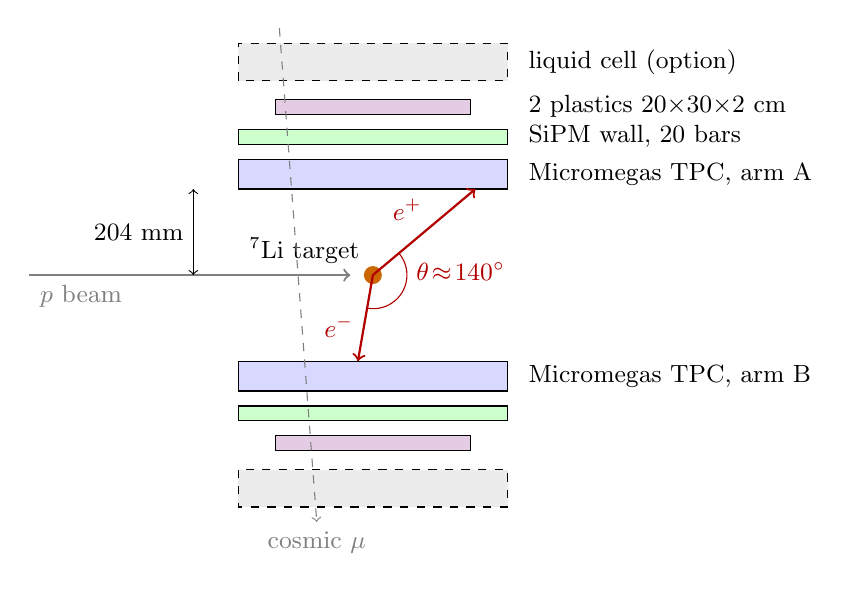
\begin{tikzpicture}[scale=0.95,font=\small]
  % beam
  \draw[->,thick,gray] (-4.6,0) -- (-0.3,0);
  \node[gray,below] at (-3.9,0) {$p$ beam};
  \fill[orange!80!black] (0,0) circle (0.12);
  \node[above left] at (-0.05,0.02) {\Li{} target};
  \foreach \s in {1,-1}{
    \begin{scope}[yscale=\s]
      \fill[blue!15] (-1.8,1.15) rectangle (1.8,1.55);  \draw (-1.8,1.15) rectangle (1.8,1.55);
      \fill[green!20] (-1.8,1.75) rectangle (1.8,1.95); \draw (-1.8,1.75) rectangle (1.8,1.95);
      \fill[violet!20] (-1.3,2.15) rectangle (1.3,2.35); \draw (-1.3,2.15) rectangle (1.3,2.35);
      \fill[gray!15] (-1.8,2.6) rectangle (1.8,3.1); \draw[dashed] (-1.8,2.6) rectangle (1.8,3.1);
    \end{scope}
  }
  \node[right] at (1.95,1.35) {Micromegas TPC, arm A};
  \node[right] at (1.95,1.85) {SiPM wall, 20 bars};
  \node[right] at (1.95,2.25) {2 plastics $20{\times}30{\times}2$~cm};
  \node[right] at (1.95,2.85) {liquid cell (option)};
  \node[right] at (1.95,-1.35) {Micromegas TPC, arm B};
  % pair, opening angle 140 deg
  \draw[->,red!70!black,thick] (0,0) -- (1.37,1.15) node[pos=0.55,above left=-1pt]{$e^+$};
  \draw[->,red!70!black,thick] (0,0) -- (-0.2,-1.15) node[pos=0.6,left]{$e^-$};
  \draw[red!70!black] (0.35,0.29) arc (40:-100:0.45);
  \node[red!70!black,right] at (0.45,0.05) {$\theta\!\approx\!140^\circ$};
  % muon
  \draw[->,gray,dashed] (-1.25,3.3) -- (-0.75,-3.3) node[below]{cosmic $\mu$};
  \draw[<->] (-2.4,0) -- (-2.4,1.15) node[midway,left]{204~mm};
\end{tikzpicture}
\caption{The two-arm configuration (view along the vertical, not to scale). Each arm: a Micromegas TPC
(30~mm drift, $399\times360$~mm$^2$ active), a wall of 20 SiPM-read plastic bars, two plastic
scintillators. The arms face each other across the beam, where the \Xs{} pairs ($\theta\approx135$--$140^\circ$)
land. A cosmic muon crosses both arms on one straight line and is rejected.}
\label{fig:setup}
\end{figure}

\paragraph{Arms.} Each arm (Fig.~\ref{fig:setup}) is, going outward from the beam axis: a Micromegas TPC
with a 30~mm drift gap and an aluminised-mylar window, its faces at $\pm204$~mm; a wall of 20
EJ-212 bars read by SiPMs; two $20\times30\times2$~cm$^3$ plastic scintillators with PMTs.
\todo{decide: two $45\times45$~cm liquid cells behind the plastics (they ran at n\_TOF; rates at LNL are far lower).}
The two chambers chosen reached 91--93\,\% efficiency within 5~mm on a cosmic bench in 2026; one needs a
drift repair and both get new windows (CEA Saclay, spring 2027).

\paragraph{Readout and trigger.} The Micromegas are read by the DREAM system (CEA; 4 FEUs and the trigger
and clock unit for two arms). The scintillators are recorded on $\sim$24 digitizer channels (16 SiPM-wall
sums, 4--6 PMTs, a trigger word). The trigger is the one used at n\_TOF: a leg per arm from the wall and
the plastics in a 20~ns coincidence; a two-arm PAIR trigger, never prescaled; SINGLE triggers prescaled by
$P = 10$--50 to monitor gains; a 1~Hz clock; DREAM's busy vetoes the trigger so that both systems keep one
event list. At LNL rates DREAM is $>95$\,\% live.

\paragraph{Target.} A thin metallic lithium film (10--12~\si{\micro\metre}, rolled and pressed onto a
backing in the argon glovebox of the LNL CN target laboratory) at the end of the beam line, in a
light end cap so that the leptons cross little material on their way to the arms.
\todo{holder: flat Al end cap at $45^\circ$ or the Cu ogive -- decide with P.~Mastinu.}
A 10--12~\si{\micro\metre} film keeps the 1.10~MeV beam above the 441~keV resonance even after partial
conversion to LiOH. Boron-free lithium is required ($^{11}$B$(p,\gamma)$ gives 16--17~MeV $\gamma$ rays).

\section{Measurements and expected precision}

\begin{enumerate}[leftmargin=1.5em]
\item \textbf{Rates and live time.} A current scan from 0.05 to 1~\si{\micro\ampere} at 1.10~MeV:
single-arm and two-arm trigger rates, DREAM live time, Micromegas occupancy and noise, the
beam-induced singles in the scintillators. Precision: scalers on every leg, $<1\,\%$ statistical in minutes.
\item \textbf{Calibration on the 17.64~MeV M1 transition} ($E_p = 441$~keV, $\Gamma_\mathrm{lab} = 12$~keV,
$\sigma \approx 5.9$~mb). Here ATOMKI saw no anomaly, so the IPC distribution is a calibration:
we expect 6--12$\times10^3$ selected pairs per day at 1~\si{\micro\ampere} with two arms, i.e.\ the
opening-angle response to $\sim$1\,\% per $10^\circ$ bin, the energy scale from the endpoint, and the
acceptance versus angle against Geant4. \todo{confirm with the two-arm re-reduction}
\item \textbf{Backgrounds.} Beam-off runs (nights, weekend) with the full trigger measure the cosmic rate
in the pair window with and without the track veto (straight, collinear segments in both chambers), the
quantity at the core of the 2026 critique of ATOMKI-type spectrometers~\cite{MEG26}. Beam-on runs measure
the accidentals and the material-induced (external) pairs.
\item \textbf{The 18.15~MeV region} ($E_p = 1.10$~MeV, five days). Rates: $\sim2\times10^3$ ground-state $\gamma$/s and
$\sim7$ IPC pairs/s into $4\pi$ per \si{\micro\ampere} for a 300~\si{\micro\gram\per\centi\metre\squared} Li$_2$O film (ATOMKI conditions); a 10--12~\si{\micro\metre} metallic film gives about 4--5 times more.
We fit the opening angle, the energy sharing and the energy sum together, with the background shape
free within the calibration. Scaling the four-arm Geant4 result to two arms, the expected 90\,\% CL
sensitivity in five days is $R \lesssim (0.8$--$1.5)\times R_\mathrm{ATOMKI}$ (Fig.~\ref{fig:reach}): the
lower value with liquid cells behind the plastics, the upper with the SiPM walls and plastics alone.
\todo{replace with the two-arm reduction (task R1); state the TOF assumption.}
\end{enumerate}

\begin{figure}[t]
\centering
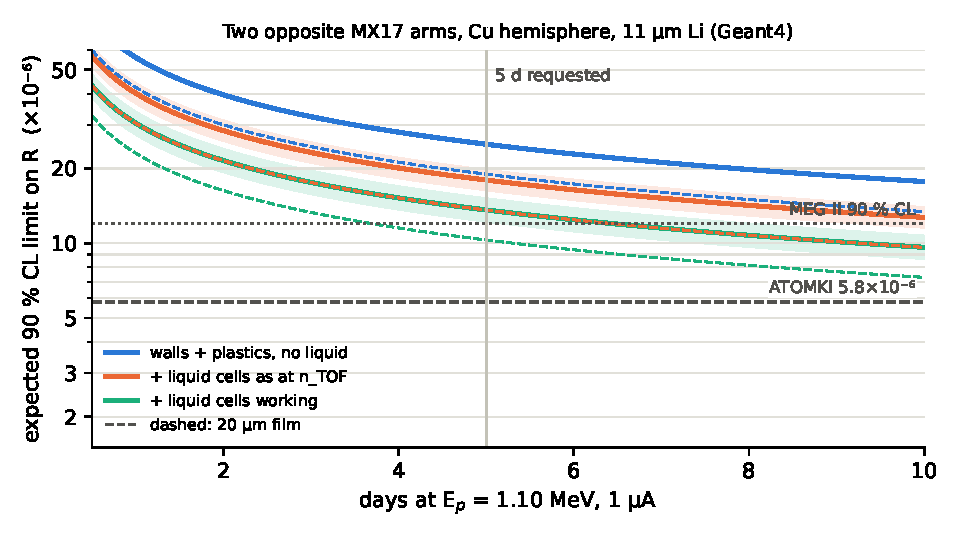
\includegraphics[width=0.82\textwidth]{figures/limit_vs_days.pdf}
\caption{Expected 90\,\% CL upper limit on $R=\Gamma_X/\Gamma_\gamma$ against days at $E_p=1.10$~MeV and
1~\si{\micro\ampere}, two opposite arms, for three energy configurations. Statistical, with the
background shape floating; bands: geometry scaling uncertainty. Scaled from the four-arm Geant4 simulation.}
\label{fig:reach}
\end{figure}

\section{Beam-time request}

\begin{table}[h]
\centering\small
\begin{tabular}{@{}llp{0.62\textwidth}@{}}
\toprule
day & $E_p$ & measurement \\
\midrule
1 & 1.10 MeV & target conditioning; current scan 0.05--1~\si{\micro\ampere}: rates, live time, occupancy \\
2--3 & 0.441 MeV & resonance located on the $\gamma$ yield; 17.64~MeV IPC calibration, 12--24k pairs \\
4--8 & 1.10 MeV & 18.15~MeV region; daily $\gamma$-yield check of the target; day 8 contingency or 0.80~MeV \\
nights & -- & beam-off cosmic runs with the full trigger \\
\bottomrule
\end{tabular}
\caption{The 8 days requested: protons, continuous, $\le 1$~\si{\micro\ampere}, three energies (one energy
change per day suits the self-service operation of AN2000).}
\label{tab:days}
\end{table}

We request \textbf{8 days of proton beam on AN2000} in the second half of 2027
(Table~\ref{tab:days}), on a line ending in about $1.5\times1.5$~m$^2$ of free floor around the target.
The CN would allow the 1.10~MeV programme but not the 441~keV calibration, below its 0.8~MV minimum.
\todo{line, floor, 24 h operation: confirm with the Accelerator Division.}

\section{From feasibility to the full experiment; requirements}

The calibration, the measured backgrounds and the timing between arms will replace the corresponding
simulation inputs and fix the full experiment: four arms, larger plastic scintillators (a factor of
13--15 in running time in simulation), and a programme on and off resonance (0.80, 1.10, 1.225~MeV).
That experiment will be the subject of a later proposal.

\textbf{Requirements and safety.} Gas: premixed Ar/iC$_4$H$_{10}$ (95/5, non-flammable-limit to be
checked) at $\sim$1~L/h with exhaust; \todo{LNL rules}. HV: Micromegas $\le 600$~V, PMTs and SiPM bias
from standard supplies. Target: metallic lithium handled in the CN target laboratory. Equipment is
owned by the collaboration or lent (CEA, INFN); installation \todo{weeks} before the beam days.

\begin{thebibliography}{9}\small
\setlength{\itemsep}{0pt}
\bibitem{Kra16} A.J.~Krasznahorkay \emph{et al.}, Phys.\ Rev.\ Lett.\ \textbf{116}, 042501 (2016).
\bibitem{Kra21} A.J.~Krasznahorkay \emph{et al.}, Phys.\ Rev.\ C \textbf{104}, 044003 (2021); review: arXiv:2409.16300 (2024).
\bibitem{Sas22} N.J.~Sas \emph{et al.}, arXiv:2205.07744 (2022).
\bibitem{Anh24} Tran The Anh \emph{et al.}, arXiv:2401.11676 (2024).
\bibitem{MEG24} MEG~II Collaboration, K.~Afanaciev \emph{et al.}, arXiv:2411.07994. \todo{journal ref}
\bibitem{MEG26} H.~Benmansour \emph{et al.}, arXiv:2609.18383 (2026).
\bibitem{GS25} B.~Góngora-Servín \emph{et al.}, Acta Phys.\ Pol.\ B Proc.\ Suppl.\ \textbf{18}, 2-A13 (2025).
\bibitem{Gus20} C.~Gustavino \emph{et al.}, \Xs{} at n\_TOF proposal \todo{CERN-INTC reference}.
\end{thebibliography}

\end{document}
